\documentclass{article}
\usepackage[paperwidth=259pt,paperheight=261pt,margin=0pt,noheadfoot]{geometry}
\usepackage{tikz}
\usetikzlibrary{calc}

\definecolor{ink}{RGB}{28,41,56}
\definecolor{axis}{RGB}{100,116,139}
\definecolor{grid}{RGB}{203,213,225}
\definecolor{curve}{RGB}{30,64,175}
\definecolor{teal}{RGB}{13,148,136}
\definecolor{tealfill}{RGB}{176,227,219}
% Integral diagrams use exactly one semantic palette: blue for the
% lower-only part, yellow for the upper-only (or still unresolved) part, and
% green for their common part.  The common part is explicit rather than an
% alpha blend, so the three meanings stay distinct after GIF quantization.
\definecolor{blue}{RGB}{0,114,178}
\definecolor{bluefill}{RGB}{86,180,233}
\definecolor{yellow}{RGB}{230,159,0}
\definecolor{yellowfill}{RGB}{255,218,102}
\definecolor{green}{RGB}{0,128,84}
\definecolor{greenfill}{RGB}{89,190,142}
\definecolor{orange}{RGB}{234,88,12}
\definecolor{orangefill}{RGB}{254,215,170}
\definecolor{purple}{RGB}{126,34,206}
\definecolor{yellowedge}{RGB}{202,138,4}
\definecolor{projection}{RGB}{148,163,184}
\colorlet{under}{blue}
\colorlet{underfill}{bluefill}
\colorlet{over}{yellow}
\colorlet{overfill}{yellowfill}
\colorlet{shared}{green}
\colorlet{sharedfill}{greenfill}
\colorlet{gap}{yellow}
\colorlet{gapfill}{yellowfill}

\pagestyle{empty}
\setlength\parindent{0pt}
\setlength\topskip{0pt}
\begin{document}
\noindent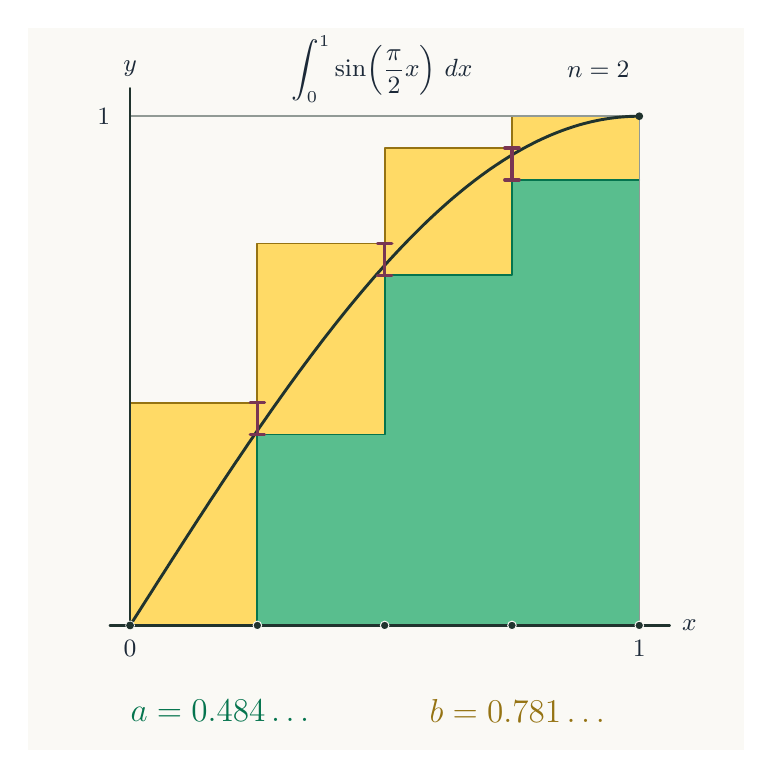
\begin{tikzpicture}[baseline=(current bounding box.north),x=1pt,y=1pt,line cap=round,line join=round]
\useasboundingbox (0,0) rectangle (259,261);
\definecolor{paper}{HTML}{FAF9F5}
\definecolor{graph}{HTML}{20332E}
\colorlet{lowerbound}{shared!85!graph}
\colorlet{upperbound}{yellow!59!graph}
\colorlet{addition}{lowerbound!76!sharedfill}
\colorlet{cutoff}{yellow!85!overfill}
\fill[paper] (0,0) rectangle (259,261);
\begin{scope}[shift={(37,45)},x=184pt,y=184pt]
\definecolor{errorbar}{HTML}{793653}
\fill[overfill] (0,0) -- (0,0.4375) -- (0.25,0.4375) -- (0.25,0.75) -- (0.5,0.75) -- (0.5,0.9375) -- (0.75,0.9375) -- (0.75,1) -- (1,1) -- (1,0) -- cycle;
\fill[sharedfill] (0,0) -- (0,0) -- (0.25,0) -- (0.25,0.375) -- (0.5,0.375) -- (0.5,0.6875) -- (0.75,0.6875) -- (0.75,0.875) -- (1,0.875) -- (1,0) -- cycle;
\draw[lowerbound,line width=.65pt] (0,0) -- (0.25,0) -- (0.25,0.375) -- (0.5,0.375) -- (0.5,0.6875) -- (0.75,0.6875) -- (0.75,0.875) -- (1,0.875);
\draw[upperbound,line width=.65pt] (0,0.4375) -- (0.25,0.4375) -- (0.25,0.75) -- (0.5,0.75) -- (0.5,0.9375) -- (0.75,0.9375) -- (0.75,1) -- (1,1);
\draw[graph!48!paper,line width=.55pt] (0,1) -- (1,1) -- (1,0);
\draw[graph,line width=.8pt] (-.04,0) -- (1.06,0);
\draw[graph,line width=.8pt] (0,0) -- (0,1.055);
\draw[graph,line width=1.05pt] plot[smooth] coordinates {(0,0) (0.0083,0.0131) (0.0167,0.0262) (0.025,0.0393) (0.0333,0.0523) (0.0417,0.0654) (0.05,0.0785) (0.0583,0.0915) (0.0667,0.1045) (0.075,0.1175) (0.0833,0.1305) (0.0917,0.1435) (0.1,0.1564) (0.1083,0.1693) (0.1167,0.1822) (0.125,0.1951) (0.1333,0.2079) (0.1417,0.2207) (0.15,0.2334) (0.1583,0.2462) (0.1667,0.2588) (0.175,0.2714) (0.1833,0.284) (0.1917,0.2965) (0.2,0.309) (0.2083,0.3214) (0.2167,0.3338) (0.225,0.3461) (0.2333,0.3584) (0.2417,0.3706) (0.25,0.3827) (0.2583,0.3947) (0.2667,0.4067) (0.275,0.4187) (0.2833,0.4305) (0.2917,0.4423) (0.3,0.454) (0.3083,0.4656) (0.3167,0.4772) (0.325,0.4886) (0.3333,0.5) (0.3417,0.5113) (0.35,0.5225) (0.3583,0.5336) (0.3667,0.5446) (0.375,0.5556) (0.3833,0.5664) (0.3917,0.5771) (0.4,0.5878) (0.4083,0.5983) (0.4167,0.6088) (0.425,0.6191) (0.4333,0.6293) (0.4417,0.6394) (0.45,0.6494) (0.4583,0.6593) (0.4667,0.6691) (0.475,0.6788) (0.4833,0.6884) (0.4917,0.6978) (0.5,0.7071) (0.5083,0.7163) (0.5167,0.7254) (0.525,0.7343) (0.5333,0.7431) (0.5417,0.7518) (0.55,0.7604) (0.5583,0.7688) (0.5667,0.7771) (0.575,0.7853) (0.5833,0.7934) (0.5917,0.8013) (0.6,0.809) (0.6083,0.8166) (0.6167,0.8241) (0.625,0.8315) (0.6333,0.8387) (0.6417,0.8457) (0.65,0.8526) (0.6583,0.8594) (0.6667,0.866) (0.675,0.8725) (0.6833,0.8788) (0.6917,0.885) (0.7,0.891) (0.7083,0.8969) (0.7167,0.9026) (0.725,0.9081) (0.7333,0.9135) (0.7417,0.9188) (0.75,0.9239) (0.7583,0.9288) (0.7667,0.9336) (0.775,0.9382) (0.7833,0.9426) (0.7917,0.9469) (0.8,0.9511) (0.8083,0.955) (0.8167,0.9588) (0.825,0.9625) (0.8333,0.9659) (0.8417,0.9692) (0.85,0.9724) (0.8583,0.9753) (0.8667,0.9781) (0.875,0.9808) (0.8833,0.9833) (0.8917,0.9856) (0.9,0.9877) (0.9083,0.9897) (0.9167,0.9914) (0.925,0.9931) (0.9333,0.9945) (0.9417,0.9958) (0.95,0.9969) (0.9583,0.9979) (0.9667,0.9986) (0.975,0.9992) (0.9833,0.9997) (0.9917,0.9999) (1,1)};
\node[font=\small,text=ink,anchor=north] at (0,-0.01) {\(0\)};
\node[font=\small,text=ink,anchor=north] at (1,-0.01) {\(1\)};
\node[font=\small,text=ink,anchor=east] at (-0.02,1) {\(1\)};
\node[font=\small,text=ink,anchor=west] at (1.065,0) {\(x\)};
\node[font=\small,text=ink,anchor=south] at (0,1.06) {\(y\)};
\filldraw[fill=graph,draw=paper,line width=.35pt] (0,0) circle[radius=1.55pt];
\filldraw[fill=graph,draw=paper,line width=.35pt] (0.25,0) circle[radius=1.55pt];
\filldraw[fill=graph,draw=paper,line width=.35pt] (0.5,0) circle[radius=1.55pt];
\filldraw[fill=graph,draw=paper,line width=.35pt] (0.75,0) circle[radius=1.55pt];
\filldraw[fill=graph,draw=paper,line width=.35pt] (1,0) circle[radius=1.55pt];
\fill[graph] (0,0) circle[radius=1.4pt];
\fill[graph] (1,1) circle[radius=1.4pt];
\draw[errorbar,opacity=1,line width=1.25pt] (0.25,0.375) -- (0.25,0.4375);
\draw[errorbar,opacity=1,line width=1.25pt] (0.236,0.375) -- (0.264,0.375);
\draw[errorbar,opacity=1,line width=1.25pt] (0.236,0.4375) -- (0.264,0.4375);
\draw[errorbar,opacity=1,line width=1.25pt] (0.5,0.6875) -- (0.5,0.75);
\draw[errorbar,opacity=1,line width=1.25pt] (0.486,0.6875) -- (0.514,0.6875);
\draw[errorbar,opacity=1,line width=1.25pt] (0.486,0.75) -- (0.514,0.75);
\draw[errorbar,opacity=1,line width=1.25pt] (0.75,0.875) -- (0.75,0.9375);
\draw[errorbar,opacity=1,line width=1.25pt] (0.736,0.875) -- (0.764,0.875);
\draw[errorbar,opacity=1,line width=1.25pt] (0.736,0.9375) -- (0.764,0.9375);
\end{scope}
\node[font=\small,text=ink] at (128,246) {\(\displaystyle\int_0^1\sin\!\left(\frac{\pi}{2}x\right)\,dx\)};
\node[font=\small,text=ink,anchor=east] at (221,246) {\(n=2\)};
\node[anchor=west,inner sep=0pt,text=lowerbound,font=\large] at (37,14) {\(a=0.484\ldots\)};
\node[anchor=west,inner sep=0pt,text=upperbound,font=\large] at (145,14) {\(b=0.781\ldots\)};
\end{tikzpicture}
\end{document}
